
% ----------------------------------------------------------------------
\section{Climate forcing}
\label{sec:climate}
% ----------------------------------------------------------------------

\subsection{Observation data}

WorldClim \citep{data:worldclim} is a high resolution climate dataset interpolated between from weather station data over global land areas. The interpolation uses 30\,arc\,s aggregated, hole-filled SRTM\needref data \todo{check WorldClim methods}, which provides a resolution much higher than attained by general circulation models.

However, the density of weather stations used by WorldClim in the Northern American Cordillera is highly inhomogeneous, and if good coverage exists in the southern parts of our modelling domain, several hundred kilometers can separate nearby stations in the north \citep{data:worldclim}.

A second drawback of the dataset in an ice sheet modelling view is the lack of data on marine surfaces, particularly on the Pacific continental shelf where glaciers have advanced during the last glacial cycle\needref.

% ----------------------------------------------------------------------

\subsection{Reanalysis data}

In addition to the WorldClim data, we use three global and one regional climate reanalysis to force the ice sheet model. Monthly climatologies from the NCEP/NCAR reanalysis\needref and the North American Regional Reanalysis (NARR)\needref were obtained from the NOAA ESRL's PSD website\needref, and monthly climatologies from the ERA-Interim\needref and Climate System Forecast Reanalyses (CFSR)\needref were computed from their monthly mean timeseries. As a mixed product of observation and circulation model, we believe that reanalysis may perform best in poorly monitored regions such as the northernmost American Cordillera. Additional information on the data used is gatherd in table \ref{tab:reanalyses}\todo{fill the table}.

\begin{table}[t]
	\caption{Characteristic of reanalysis data used as a forcing for the ice sheet model.}
	\label{tab:reanalyses}
	\vskip4mm
	\centering
	\begin{tabular}{lllll}
		\tophline
		Reanalysis& coverage& time period&  resolution& reference\\
		\middlehline
		NCEP/NCAR&  global&   1981 -- 2010& ??& ??\\
		ERA-Interim&global&   1979 -- 2011& ??& ??\\
		CFSR&       global&   1979 -- 2010& ??& ??\\
		NARR&       global&   1979 -- 2000& ??& ??\\
		\bottomhline
	\end{tabular}
\end{table}

% ----------------------------------------------------------------------

\subsection{Cordillera climates}

\begin{figure}[t]
	\vspace*{2mm}
	\begin{center}
		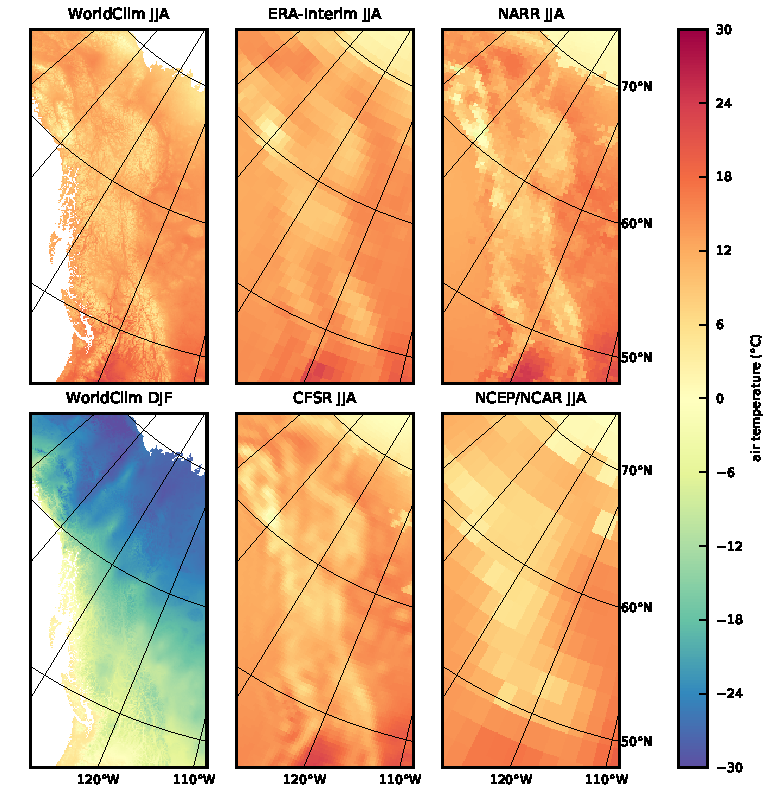
\includegraphics[width=13cm]{cordillera-climate-temp}
	\end{center}
	\caption{Summer temperature maps from the five datasets used in this study and winter temperature map from the WorldClim dataset.}
	\label{fig:temp}
\end{figure}

\begin{figure}[t]
	\vspace*{2mm}
	\begin{center}
		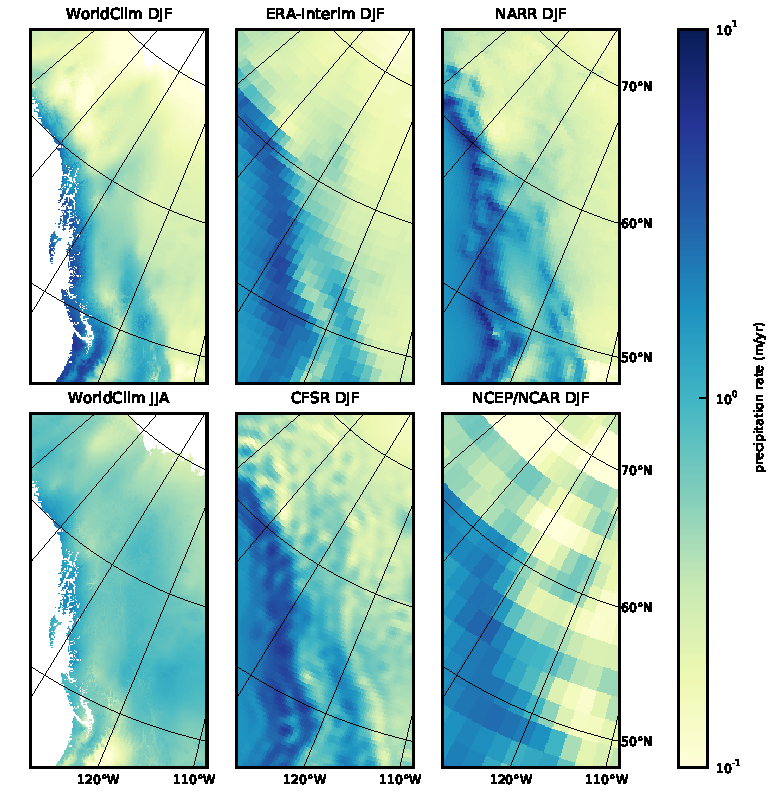
\includegraphics[width=13cm]{cordillera-climate-prec}
	\end{center}
	\caption{Winter precipitation rate maps from the five datasets used in this study and summer precipitation map from the WorldClim dataset.}
	\label{fig:prec}
\end{figure}

% ----------------------------------------------------------------------

\subsection{Preprocessing and lapse-rate corrections}

\begin{figure}[t]
	\vspace*{2mm}
	\begin{center}
		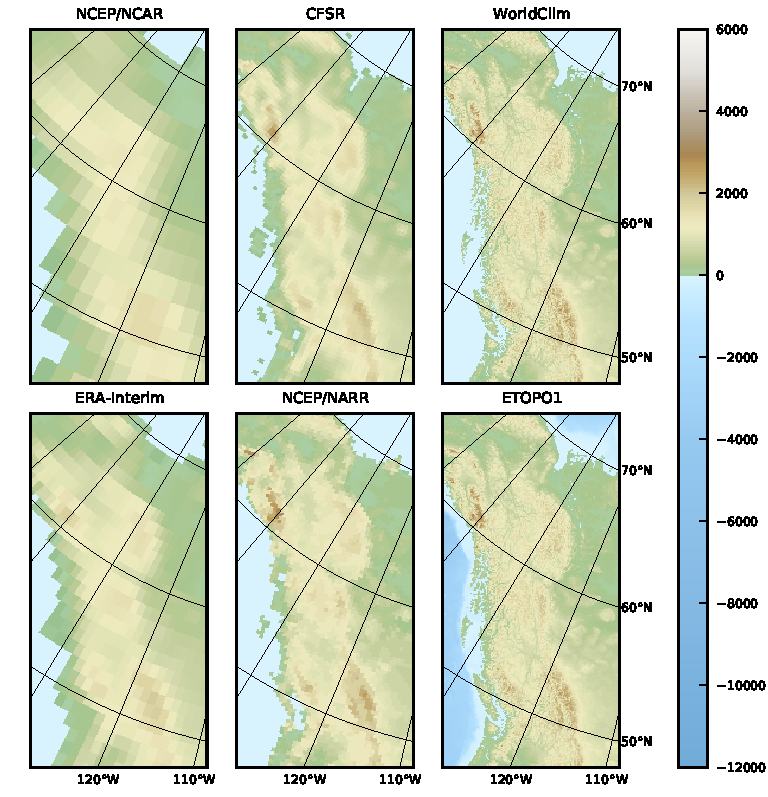
\includegraphics[width=13cm]{cordillera-climate-topo}
	\end{center}
	\caption{Reference topography used for temperature lapse-rate corrections from the five climate datasets used in the study and ETOPO1 topography used as basal condition for the ice flow model.}
	\label{fig:topo}
\end{figure}

